\chapter{Limits and colimits}
So far, we've been building a ``categorical dictionary'' of structure that
categories might have that makes them useful models for programming languages.
Categorical products let us model products in programming languages, exponential
objects let us model higher-order functions. Limits and colimits take these
ideas to their extreme: we will see that a category that has limits and colimits
has a rich vocabulary of universal constructions of which products and
exponentials are a special case. The utility of limits and colimits is in their 
generality, both in the kinds of constructions they give you and also how they
are characterized. We will see that limits are \emph{preserved} or
\emph{created} by the presence of certain functors, enabling us to characterize
a large amount of categorical structure with relatively little work. 

As an example of how limits generalize products, let
\[
\mathsf{Point} = \{
x: \R, y: \R, z: \R
\}
\]
This leads to the idea of indexed products.
\begin{definition}[Indexed product]
  \sloppy
  Let \((X_i)_{i\in I}\) be an \(I\)-indexed
  family of objects of a category \(\calC\).
  An \emph{indexed product} of \((X_i)_{i\in I}\)
  consists of an object \(P\)
  and a family of morphisms \((\pi_i : P \to X_i)_{i\in I}\)
  satisfying the following universal property:
  for any object \(Y\)
  and any family of morphisms \((f_i : Y \to X_i)_{i\in I}\),
  there exists a unique morphism \(\angled{f_i}_{i\in I} : Y \to P\)
  such that \(\pi_i \circ \angled{f_i}_{i\in I} = f_i\) for all \(i\) in \(I\).
\end{definition}
While records are typically finite, the definition of indexed product
works just as well for infinite products.
For example,
\begin{proposition}
  \(1\) is the indexed product of \((k)_{k\in \N}\)
  in the category of natural numbers under divisibility.
\end{proposition}
More generally, indexed products in preorders are like infima.

Indexed products are in some sense the ``largest'' way to map
into a tuple of objects.
For example, the product for \(\mathsf{Point}\)
is the ``largest'' way of filling in the question marks in this diagram:
\[% https://tikzcd.yichuanshen.de/#N4Igdg9gJgpgziAXAbVABwnAlgFyxMJZABgBoBGAXVJADcBDAGwFcYkQAdDgJRAF9S6TLnyEU5CtTpNW7LrwFDseAkQBMkmgxZtEnHv0EgMy0UQnEp22XoD8-KTCgBzeEVAAzAE4QAtkgBmGhwIJDJpHXZ7GkZ6ACMYRgAFYRUxEC8sZwALHENPH39EIJAQpAkImxB7RRBvP0Dg0MQNSt1qhz4gA
\begin{tikzcd}
   & ? \arrow[ld, "?"'] \arrow[d, "?"] \arrow[rd, "?"] &    \\
\R & \R                                                & \R
\end{tikzcd}\]
Similarly, \(1\) is the ``largest'' way to fill in
the question marks in this diagram:
\[% https://tikzcd.yichuanshen.de/#N4Igdg9gJgpgziAXAbVABwnAlgFyxMJZARgBpiBdUkANwEMAbAVxiRAH4QBfU9TXfIRQAGUsKq1GLNsW68QGbHgJEy46vWatEIAExy+SwUV1iJm6ToDMBhf2VDkVsxqnaQAHQ9QIOBFwkYKABzeCJQADMAJwgAWyRREBwIJDJJLTZOHkiY+MRE5KRTdMsOW2i4hOpCxGcS9yz5CryClMQAFlcMnU5qBjoAIxgGAAV7Yx0orGCACxxuCi4gA
\begin{tikzcd}
1 & 2                                                                  & 3 & \dots \\
  & ? \arrow[lu, "?"] \arrow[u, "?"] \arrow[ru, "?"] \arrow[rru, "?"'] &   &
\end{tikzcd}\]

All of these diagrams are ``discrete'': they consist only of objects,
with no morphisms connecting them.
More generally, we can ask if it is possible to find the largest
way of mapping into an arbitrary diagram consisting of both objects and morphisms.
This is called a \emph{limit}.

To be more precise about this, it is useful to give a formal definition of 
what a diagram is:
\begin{definition}[Diagram]
  \sloppy
  For two categories $\calI$ and $\calC$, a
  \emph{diagram of shape $\calI$} is a functor $F : \calI \to \calC$.
  The category $\calI$ is called the \emph{shape of the diagram}.
\end{definition}

It is typical for the shape of a diagram to be a simple discrete category with
only a few objects and morphisms.  For example, we can consider $\calI = \bullet
\quad \bullet$; then, a diagram of shape $\calI$ in some category $\calC$ would
pick out a pair of two objects in $\calC$. Here is a simple example of a
diagram:

\begin{center}
  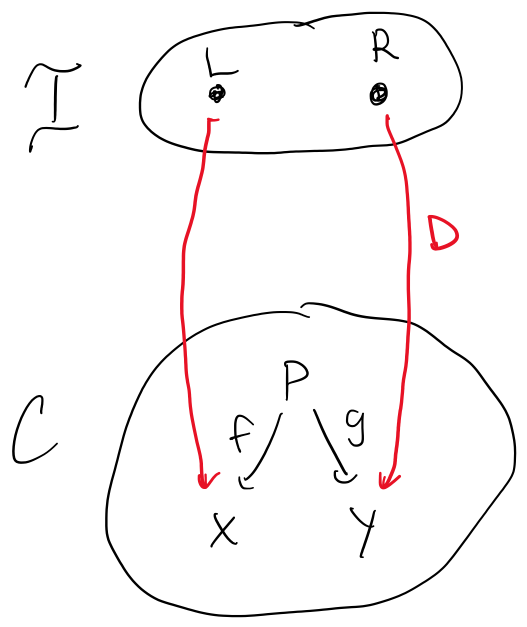
\includegraphics[width=100px]{fig/diagram-1.png}
\end{center}

The essential idea of a limit is that it that it is the largest way of ``mapping 
into a diagram''. 
The way to formalize this is via the notion of a \emph{cone}:

\begin{definition}[Cone]
  \sloppy
  Let \(D : \mathcal I \to \calC\) be a diagram of shape \(\mathcal I\)
  in a category \(\calC\).
  A \emph{cone} over \(D\) is a pair \((P,p)\)
  where \(P\) is an object of \(\calC\)
  and \(p\) is a family of morphisms \((p_i : P \to D(i))_{i\in I}\)
  such that \(D(f) \circ p_i = p_j\) for all morphisms \(f : i \to j\)
  of \(\mathcal I\).
\end{definition}

Let's understand this definition for the simple diagrams of shape $\calI =
\bullet \quad \bullet$ before we consider more more interesting shapes with
morphisms in them. In the above example diagram, the tuple $(P, p)$
is a cone where $p_L = f$ and $p_R = g$.


Cones form a category:
\begin{definition}
  Let \(D : \mathcal I \to \calC\) be a diagram of shape \(\mathcal I\)
  in a category \(\calC\).
  Let \((P,p)\) and \((Q,q)\) be two cones over \(D\).
  A \emph{morphism of cones from \((P,p)\) to \((Q,q)\)}
  is a morphism \(f : P \to Q\) such that \(f \circ p_i = q_i\)
  for all \(i \in \mathcal I\).
\end{definition}
A morphism of cones can be visualized as a kind of 3d prism:
\[% https://tikzcd.yichuanshen.de/#N4Igdg9gJgpgziAXAbVABwnAlgFyxMJZARgBpiBdUkANwEMAbAVxiRABEAKLAShAF9S6TLnyEUZAExVajFmy4ArPoOHY8BIpNIAGGfWatEIAIoChIDOrFEdu-XKMgACgJkwoAc3hFQAMwAnCABbJDsQHAgkYlUQQJCkAGZqSKRtWUM2P3N-INDEdNTEcIN5YwBHAH0sEGoGOgAjGAZnEQ1xEACsTwALHBy4vLSUqMQyDLKQKsUB+PzkiNHwprAoMOpSpzRq2pB6ppa2m2MGGD9+2LmkkeiNxzZtmbrG5tbrTWMu3ouKfiA
\begin{tikzcd}
P \arrow[rr, "f"] \arrow[rd, "p_i"] \arrow[rdd, "p_j"'] &                & Q \arrow[ld, "q_i"'] \arrow[ldd, "q_j"] \\
                                                        & D(i) \arrow[d] &                                         \\
                                                        & D(j)           &
\end{tikzcd}\]
At the bottom of this prism, we have drawn a piece of the diagram \(D\).
The ``bottom left face'' of the prism is the cone \((P,p)\); the ``bottom right face'' is the cone \((Q,q)\).
A morphism of cones from \((P,p)\) to \((Q,q)\) is a morphism \(f : P \to Q\) as shown
that makes all the triangles in the prism commute.

Looking at specific choices of diagram \(D\) recovers the kinds of figures we were drawing.
For example, suppose
\(D\) is the discrete diagram on two objects \(X\) and \(Y\). We get that
  a cone \((P,p)\) is a diagram of shape \[% https://tikzcd.yichuanshen.de/#N4Igdg9gJgpgziAXAbVABwnAlgFyxMJZABgBoBGAXVJADcBDAGwFcYkQANEAX1PU1z5CKAEwVqdJq3YBNHnxAZseAkXKliEhizaIQABR4SYUAObwioAGYAnCAFskYkDghIyknezQB9ciBpGegAjGEZ9ARVhEBssUwALHHlrO0dEZ1ckdU9pPV8RI24gA
\begin{tikzcd}
  & P \arrow[ld, "p_1"'] \arrow[rd, "p_2"] &   \\
X &                                        & Y
\end{tikzcd}\]
and a morphism from one such cone \((P,p)\) to another \((Q,q)\)
is a diagram of shape:
\[% https://tikzcd.yichuanshen.de/#N4Igdg9gJgpgziAXAbVABwnAlgFyxMJZARgBpiBdUkANwEMAbAVxiRAA0QBfU9TXfIRRkATFVqMWbAJrdeIDNjwEiI0gAZx9Zq0QgAinL5LBRdRq2TdIAArdxMKAHN4RUADMAThAC2SAMzUOBBIahI6bO5GIF6+oUEhiObhUnoAjgD6WCDUDHQARjAMNvzKQiCeWE4AFjjRsX6IYcFIZCnWmQBW9d6NgSAtSdSFYFBIydqpClk5IHmFxaWmegww7nU8Hr0BCa3Uk9ZoGd25BUUlJip6lTUbFFxAA
\begin{tikzcd}
P \arrow[rr, "f"] \arrow[rd, "p_i"] \arrow[rdd, "p_j"'] &   & Q \arrow[ld, "q_i"'] \arrow[ldd, "q_j"] \\
                                                        & X &                                         \\
                                                        & Y &
\end{tikzcd}\]
Now imagine taking the object \(P\) and ``dragging it up and to the right'', until it's in the same plane
as the triangle involving \(Q,X,Y\):
\[% https://tikzcd.yichuanshen.de/#N4Igdg9gJgpgziAXAbVABwnAlgFyxMJZABgBoAmAXVJADcBDAGwFcYkQANEAX1PU1z5CKMgGZqdJq3YBNHnxAZseAkQCMpNRIYs2iEAEV5-ZUKLlSxbVL0gACjwkwoAc3hFQAMwBOEALZIojQ4EEgWkrrsnsYgPv5hwaGIZBHS+gCOAPpYIDSM9ABGMIx2AirCIN5YLgAWODFxAYjhIUgaqbZZAFYNvk1BIK3JNEVgUEgAtKIpOmmK2bkg+UUlZWb6VbX1vF59gYltNLO2aJk9eYXFpaaq+owwnvUjMGOBxNyU3EA
\begin{tikzcd}
  &                                         & P \arrow[ld, "f"] \arrow[lldd, "p_i"', bend right] \arrow[llddd, "p_j", bend left] \\
  & Q \arrow[ld, "q_i"'] \arrow[ldd, "q_j"] &                                                                                    \\
X &                                         &                                                                                    \\
Y &                                         &
\end{tikzcd}\]
Hopefully this diagram looks familiar: up to a rotation, it is the kind of diagram we were drawing when examining
the universal property of product.

Together, cones over a diagram \(D\) and morphisms between them form a category:
\begin{definition}[category of cones]
  Let \(D :\mathcal I \to \calC\) be a diagram in a category \(\calC\) of shape \(\mathcal I\).
  The category of cones over \(D\), written \(\mathsf{Cone}(D)\),
  is the category whose objects are cones over \(D\) and whose morphisms are morphisms of cones.
  (Because cone morphisms are simply morphisms of \(\calC\) satisfying a certain property,
   the definition of composition for cone morphisms and of the identity cone morphism are inherited from
   composition and identity in \(\calC\).)
\end{definition}

\begin{definition}[Limit]
  Let \(D : \mathcal I \to \calC\) be a diagram of shape \(\mathcal I\)
  in a category \(\calC\).
  A \emph{limit} of \(D\) is a terminal cone.
\end{definition}



\section{Examples of limits}

We have seen two examples of limits already, in the homework.
\begin{itemize}
\item Given two morphisms \(X \mor{f} Z \xleftarrow{g} Y\),
  the \emph{pullback} is the largest way of mapping into \(f,g\),
  in other words the largest way of filling in the question marks in this
  diagram:
  \[
  % https://tikzcd.yichuanshen.de/#N4Igdg9gJgpgziAXAbVABwnAlgFyxMJZABgBoBGAXVJADcBDAGwFcYkQANEAX1PU1z5CKcqWLU6TVuwCaPPiAzY8BIqKo0GLNohAAtef2VCiZcZqk6QAfh4SYUAObwioAGYAnCAFskAZhocCCQySW12WxpGegAjGEYABQEVYRAPLEcACxxDEE8ff0DgxFEw6V1bXncvXxKipAAmC3DdR1z82tCgxubyvJAo2Pik41VddKyc7kpuIA
\begin{tikzcd}
? \arrow[d, "?"'] \arrow[r, "?"] & Y \arrow[d, "g"] \\
X \arrow[r, "f"']                & Z
\end{tikzcd}
  \]
  Explicitly, a pullback is a 3-tuple \((W,p,q)\)
  where \(p : W \to X\) and \(q : W \to Y\)
  and \(fp = gq\)
  satisfying the following universal property:
  for any other 3-tuple \((W',p',q')\)
  where \(p' : W' \to X\) and \(q' : W' \to Y\)
  and \(fp' = gq'\),
  there exists a unique morphism \(w : W' \to W\)
  such that \(pw = p'\) and \(qw = q'\).
  \[% https://tikzcd.yichuanshen.de/#N4Igdg9gJgpgziAXAbVABwnAlgFyxMJZARgBoAmAXVJADcBDAGwFcYkQANEAX1PU1z5CKcqWLU6TVuwCaPPiAzY8BIqKo0GLNohAAtef2VCiZcZqk6QAdUOKBK4cgAMpZxK3Td1gOQ8JMFAA5vBEoABmAE4QALZIAMw0OBBIrpLa7GggNIz0AEYwjAAKDia6kVhBABY4dlGxCUkpiGTpXiAAjnXRcS1NSKJtVkHdDYhpyQMWGbrh2SC5BcWlquWVNaO9ACz94zQFYFBIALTxaZ5WXTn5hSXGqyAV1bW8ET1IOyCTfSAHR4hnabtDp+V4gerbXaJIbsADu-m4QA
\begin{tikzcd}
W' \arrow[rdd, "q"', bend right] \arrow[rrd, "q'", bend left] \arrow[rd, "w"] &                                  &                  \\
                                                                              & W \arrow[d, "p"'] \arrow[r, "q"] & Y \arrow[d, "g"] \\
                                                                              & X \arrow[r, "f"']                & Z
\end{tikzcd}\]
\item Given two morphisms \(% https://tikzcd.yichuanshen.de/#N4Igdg9gJgpgziAXAbVABwnAlgFyxMJZABgBpiBdUkANwEMAbAVxiRAA0QBfU9TXfIRQBGclVqMWbAJrdxMKAHN4RUADMAThAC2SMiBwQkokHAAWWNTmPV6zVohCKQ1BnQBGMBgAV+eAmwaWIpm1jzqWrqI+oY2EvZsai6mFlZIALTCXBRcQA
\begin{tikzcd}
X \arrow[r, "g"', shift right] \arrow[r, "f", shift left] & Y
\end{tikzcd}\),
their \emph{equalizer} is the largest way of mapping into \(f,g\)
in other words the largest way of filling in the questino marks in this
diagram:
\[% https://tikzcd.yichuanshen.de/#N4Igdg9gJgpgziAXAbVABwnAlgFyxMJZABgBoBGAXVJADcBDAGwFcYkQANEAX1PU1z5CKAEwVqdJq3YBNHnxAZseAkXKliEhizaIQAfh4SYUAObwioAGYAnCAFskZEDghJ1IOAAssVnO5ptaT1TEBpGegAjGEYABQEVYRAbLFMvf15rO0dEZ1cAyR12KzDPHz8kAFpyTJBbByQxFzdcwKldA1KI6LiEoXYUtIyFepym-MQPII7DbkpuIA
\begin{tikzcd}
                                                            & ? \arrow[ld, "?"'] \arrow[rd, "?"] &   \\
X \arrow[rr, "g"', shift right] \arrow[rr, "f", shift left] &                                    & Y
\end{tikzcd}\]
Explicitly, the equalizer is a 3-tuple \((W,p,q)\)
where \(p : W \to X\) and \(q : W \to Y\)
and \(fp = q\) and \(gp = q\)
satisfying the following universal property:
for any other 3-tuple \((W',p',q')\)
where \(p' : W' \to X\) and \(q' : W' \to Y\)
and \(fp' = q'\) and \(gp' = q'\)
there exists a unique \(w : W' \to W\)
such that \(pw = p'\) and \(qw = q'\).
\[% https://tikzcd.yichuanshen.de/#N4Igdg9gJgpgziAXAbVABwnAlgFyxMJZABgBoAmAXVJADcBDAGwFcYkQANEAX1PU1z5CKchWp0mrdgE0efEBmx4CRAIylV4hizaIQAdTn8lQtaWJbJugwHIe4mFADm8IqABmAJwgBbJGRAcCCR1EDgACyx3HBCabSk9JxAaRnoAIxhGAAUBZWEQTywncJjeD28-RACg2IkddndksMjopABaVTKQL18kUUDgqrirdjQm1Izs3NM9QuLS+R7K-prEUPjrAEcjboqkAGYaVYCN0bsU9MyckxVZopKmjLAodv3iLqWDo8H1kb1N84gJ4vRBvD57UHfPrDep6ADu9m4QA
\begin{tikzcd}
                                                            & W' \arrow[ldd, "p'"', bend right] \arrow[rdd, "q'", bend left] \arrow[d, "w"] &   \\
                                                            & W \arrow[ld, "p"'] \arrow[rd, "q"]                                            &   \\
X \arrow[rr, "g"', shift right] \arrow[rr, "f", shift left] &                                                                               & Y
\end{tikzcd}\]
This definition can be simplified a bit:
notice that in the 3-tuple \((W,p,q)\),
the morphism \(q\) is forced to be \(fp\).
So it is equivalent to say that an equalizer
is a 2-tuple \((W,p)\)
such that \(fp = gp\),
which satisfies the universal property
that for any other \((W',p')\)
with \(fp' = gp'\), there exists a unique \(w : W' \to W\)
such that \(wp = p'\) and \(wq = q'\).
\[% https://tikzcd.yichuanshen.de/#N4Igdg9gJgpgziAXAbVABwnAlgFyxMJZARgBpiBdUkANwEMAbAVxiRAA0QBfU9TXfIRQAmclVqMWbAJrdeIDNjwEiABjHV6zVohAB1OXyWC1pVeK1TdegOTdxMKAHN4RUADMAThAC2SdSA4EEhkEtps7iDUcAAWWO44SAC0xDwe3n6IAUEhmpI6IE5RILHxiYihDHQARjAMAAr8ykIgnlhOMYlpIF6+SKKBwVl54bpohj0ZSADM1DnDYVYKdt29mbOD-SNLAO7FVbUNTSa6bR1dFFxAA
\begin{tikzcd}
W' \arrow[rd, "p'"] \arrow[d, "w"'] &                                                           &   \\
W \arrow[r, "p"]                    & X \arrow[r, "f", shift left] \arrow[r, "g"', shift right] & Y
\end{tikzcd}\]
\end{itemize}

The equalizer looks like a refinement type:
\[
\text{equalizer of }
\begin{tikzcd}
X \arrow[r, "g"', shift right] \arrow[r, "f", shift left] & Y
\end{tikzcd}
\qquad\leadsto\qquad
\{x : X \mid f(x) = g(x)\}
\]

The pullback looks like a ``fiber product'':
\[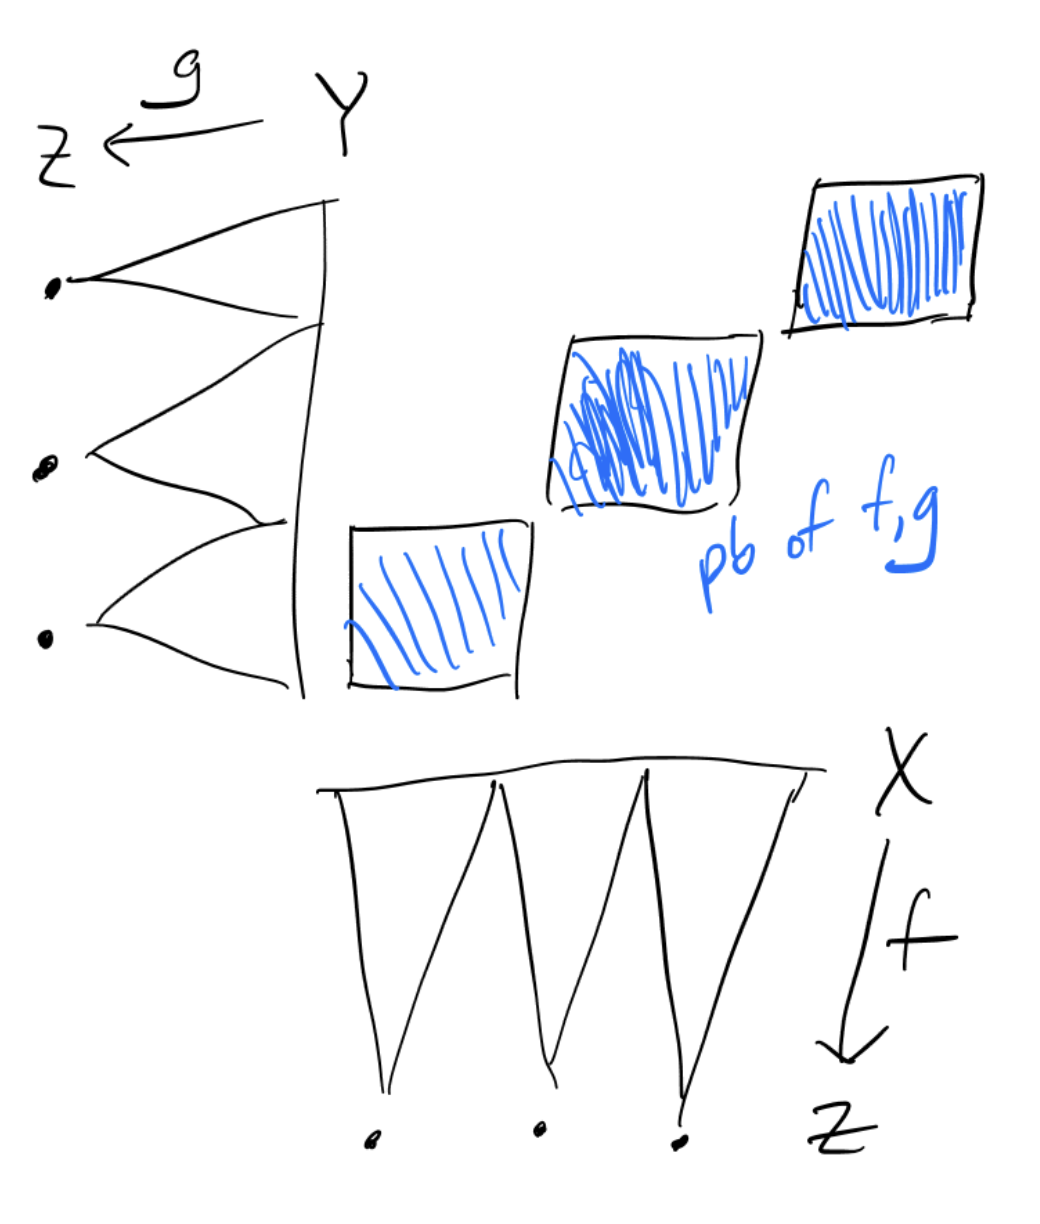
\includegraphics[width=100px]{fig/pb.png}\]


There is an equivalent way of defining cones, that requires a bit more machinery.

\begin{definition}
  Given an object \(X\) of a category \(\calC\),
  and an arbitrary category \(\mathcal I\),
  the \emph{constant functor at \(X\) from \(\mathcal I\) to \(\calC\)},
  written \(\Delta(X) : \mathcal I \to \calC\),
  is the functor defined by
  \(\Delta(X)(i) = X\) on objects \(i\) of \(\mathcal I\)
and by \(\Delta(X)(i \mor{f} j) = \mathsf{id}_X\) on morphisms.
\end{definition}

\begin{proposition}
  A cone over \(D : \mathcal I \to \calC\) is equivalent to a pair \((P,\alpha)\)
  where \(P\) is an object of \(\calC\) and \(\alpha\) is a natural transformation
  \(\Delta(P) \Rightarrow D\).
\end{proposition}
\begin{proof}
  Unwinding definitions, the natural transformation \(\alpha\) is a \(\mathcal I\)-indexed family
  of morphisms \((\alpha_i : \Delta(P)(i) \to D(i))_{i\in \mathcal I}\)
  satisfying the following naturality square for all morphisms \(i\mor{f} j\) of \(\mathcal I\):
  \[
  % https://tikzcd.yichuanshen.de/#N4Igdg9gJgpgziAXAbVABwnAlgFyxMJZABgBpiBdUkANwEMAbAVxiRAB12ARGBnOgBQAFAJQCsIkAF9S6TLnyEUZAIxVajFm048+g0QIBWkmXOx4CRFaTXV6zVohBcjJ2SAznFV8uvtanFwlpdRgoAHN4IlAAMwAnCABbJDIQHAgkaw0HbW5efmExGMlqBjoAI14heQslEDiscIALHGl3eKSU6nSkAGY7TUcOdkY0JroAfSw22ITkxCyexAAmAZynTlHxicMQUoqqmu8nBubW0xAO+f60jJW1gOcBYpCpIA
\begin{tikzcd}
\Delta(P)(i) \arrow[d, "\Delta(P)(f)"'] \arrow[r, "\alpha_i"] & D(i) \arrow[d, "D(f)"] \\
\Delta(P)(j) \arrow[r, "\alpha_j"']                           & D(j)
\end{tikzcd}
  \]
  But by definition of \(\Delta(P)\), it holds that \(\Delta(P)(i) = \Delta(P)(j) = P\)
  and \(\Delta(P)(f) = \mathsf{id}_P\).
  Hence the left arrow in this commutative square is the identity,
  and the square can be collapsed into the following triangle which has to commute for all \(i\mor{f} j\) in \(\mathcal I\):
  \[
  % https://tikzcd.yichuanshen.de/#N4Igdg9gJgpgziAXAbVABwnAlgFyxMJZABgBoBGAXVJADcBDAGwFcYkQAFEAX1PU1z5CKcqWLU6TVuwAiACiwBKHnxAZseAkVEAmCQxZtEIeQCtl3CTCgBzeEVAAzAE4QAtkjIgcEJKMmG7AA6QUxoABb0APpYKk6uHohePkg6NAbSxiFhkVGmIDSM9ABGMIwcAprCIM5YNuE4cSAu7n40KYhpAZkmco4WlNxAA
\begin{tikzcd}
                                                 & D(i) \arrow[dd, "D(f)"] \\
P \arrow[ru, "\alpha_i"] \arrow[rd, "\alpha_j"'] &                         \\
                                                 & D(j)
\end{tikzcd}
  \]
  Hence the natural transformation \(\alpha : \Delta(P) \Rightarrow D\)
  amounts to a family of morphisms \((\alpha_i : P \to D(i))_{i\in \mathcal I}\)
  satisfying the property that \(D(f) \circ \alpha_i = \alpha_j\) for all \(i \mor{f} j\) in \(\mathcal I\).
  This is precisely the property of being a cone over \(D\).
\end{proof}

Last time we saw by the Yoneda lemma that a representation for a \(\calC\)-indexed set \(P\)
is equivalent to a terminal object in \(\int P\), the category of elements of \(P\).
This fact provides an interesting equivalent definition of limit:
\begin{proposition}
  Let \(\mathcal I\) be a \(\calU\)-small category.
  A limit of a diagram \(D : \mathcal I \to \calC\)
  is equivalent to a reprsentation for the \(\calC\)-indexed set \(P\) defined by
  \[
     P(X) = \text{the set of natural transformations }\Delta(X) \Rightarrow D.
  \]
\end{proposition}
\begin{proof}
  The \(\calC\)-indexed set \(P\) is designed so that
  the category of cones over \(D\) is equivalent to the category of elements of \(P\).
  Hence, to have a terminal cone is to have a terminal object in this category of elements,
which is equivalent to having a representation for \(P\).
\end{proof}


\subsection{Some important facts}

\begin{itemize}
\item Homework 2 Problem 3
\item Universal element definition of limit
\item Every limit is an equalizer of a product.
\item Equalizers as refinement types; limits as refinement types + indexed products
\item Limits in Set
\item The Yoneda embedding preserves limits
\item Any full and faithful functor reflects limits and colimits.
\end{itemize}
